\documentclass{config/apuntes}

\title{Redes Biológicas y Biología de Sistemas}
\author{Sandra Mingo Ramírez}
\date{2024/25}
\acronym{RBBS}

\usepackage[all]{nowidow}
\usepackage{listing}
\usepackage{color}
\usepackage{tabularx}
\usepackage{multirow}
\usepackage{makecell}
\usepackage{amsmath}
\usepackage{array}
\usepackage{soul}

\definecolor{dkgreen}{rgb}{0,0.6,0}
\definecolor{gray}{rgb}{0.5,0.5,0.5}
\definecolor{mauve}{rgb}{0.58,0,0.82}

\lstset{
  frame=tb,
  aboveskip=3mm,
  belowskip=3mm,
  showstringspaces=false,
  columns=flexible,
  basicstyle={\small\ttfamily},
  numbers=none,
  numberstyle=\tiny\color{gray},
  keywordstyle=\color{blue},
  commentstyle=\color{dkgreen},
  stringstyle=\color{mauve},
  breaklines=true,
  breakatwhitespace=true,
  tabsize=3
}

\usepackage{tocloft}

\advance\cftchapnumwidth 0.9em\relax
\advance\cftsecnumwidth 0.6em\relax
\advance\cftsubsecindent 0.5em\relax
\advance\cftsubsecnumwidth 0.5em\relax
\begin{document}

\begin{abstract}
La biología de sistemas busca entender la importancia de cuantificar en biología y poder formular algunos problemas biológicos en modelos matemáticos relativamente simples. Los modelos son siempre simplificaciones grandes de los sistemas biológicos complejos. Muchas veces, esas simplificaciones no son abstractas, si no que reflejan el conocimiento que se tiene de los sistemas. No obstante, todos son imperfectos, ya que no contienen toda la información posible. Como decía el estadístico George Box, todos los modelos son erróneos, pero algunos son útiles. Por eso, en esta asignatura aprenderemos a cuantificar en biología y construir modelos matemáticos.
\end{abstract}

\pagestyle{plain}

\maketitle

\tableofcontents

%GUÍA DOCENTE
%Ejercicios 60%
%Memoria 15%
%Defensa 15%
%Participación 10%

%50% Teoría: 40% examen preguntas cortas/problemas, 60% projecto en grupo
%50% Prácticas: 

%30/01 - Raúl Guantes
\chapter{Conceptos básicos}
\section{La importancia de cuantificar y estimar las escalas en biología}
La biología de sistemas es un campo que busca entender los sistemas biológicos a través de la cuantificación y la modelización matemática. Los modelos matemáticos son simplificaciones de sistemas biológicos complejos, y aunque no son perfectos (ya que no pueden capturar toda la información), son útiles para entender y predecir comportamientos biológicos. Como dijo el estadístico George Box: "Todos los modelos son erróneos, pero algunos son útiles".

Una herramienta clave en este campo es BioNumbers, una base de datos que recopila información cuantitativa en biología. Esta información es esencial para interpretar resultados experimentales y diseñar nuevos experimentos. Por ejemplo, al realizar experimentos, es fundamental calcular la media y la desviación estándar de los resultados para estimar el error. El error se redondea a una cifra significativa, y la medida se expresa con la misma precisión que el error.

\subsection{Estimación de la expresión de proteínas en \textit{E. coli}}
Supongamos que encontramos una proteína en un cultivo celular de \textit{E. coli} con una concentración de 1 picoMolar (pM) por célula. ¿Es esta expresión significativa? Para responder, necesitamos calcular el número de moléculas de la proteína por célula, lo que depende del volumen celular.

\paragraph{Datos} Las bacterias tienen forma cilíndrica con una longitud de 2 micras y un diámetro de 1 micra. La concentración de la proteína: $C = 1 pM = 10^{-12}M$.

\paragraph{Cálculos}
\begin{enumerate}
\item Volumen de la célula
$$V = \pi r^2 h \rightarrow \pi (0,5 \mu m)^2 2 \approx 1,5 \mu m^3 = 1,5 \cdot 10^{-15} l = 1,5 fl$$
\item Número de moléculas de proteína por célula
$$C = \frac{N_p}{V \cdot N_{av}} \rightarrow N_p = C \cdot V \cdot N_{av}$$
$$N_p = C \cdot V \cdot N_{av} = 10^{-12}M \cdot 1,5 \cdot 10^{-15}l \cdot 6 \cdot 10^{23} \approx 10^{-3} molecules$$
Esto significa que hay aproximadamente 1 molécula de proteína por cada 1.000 células.
\end{enumerate}

De esta forma, podemos decir que como regla general, una concentración de 1 nanomolar (nM) en \textit{E. coli} corresponde aproximadamente a 1 molécula por célula, dado que el volumen de una célula de \textit{E. coli} es del orden de 1 fl.

\subsection{Variabilidad en la cuantificación de proteínas}
En \textit{E. coli}, la cantidad de proteínas se ha cuantificado utilizando dos técnicas principales: espectrometría de masas y microscopía de fluorescencia. Estas técnicas arrojan resultados diferentes:
\begin{itemize}
\item En espectrometría de masas, el número promedio de una proteína cualquiera en \textit{E. coli} es de 1.000-2.000 moléculas.
\item En microscopía de fluorescencia, este número es de alrededor de 50 moléculas.
\end{itemize}

\begin{figure}[h]
\centering
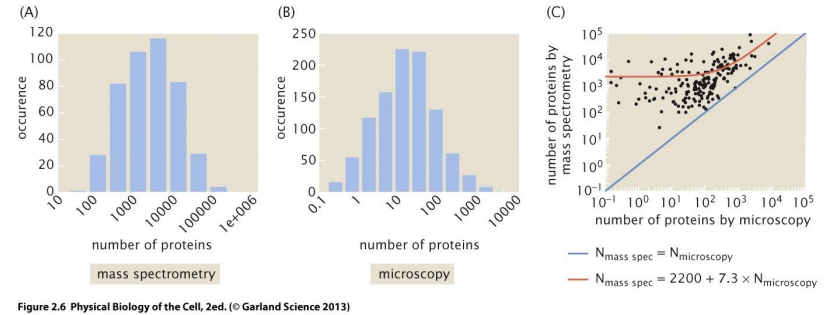
\includegraphics[width = 0.9\textwidth]{figs/mol-census.png}
\end{figure}

Para \textbf{proteínas muy abundantes}, ambas técnicas muestran una buena correlación.
Para \textbf{proteínas poco abundantes}, la correlación se pierde debido a la variabilidad intrínseca en la expresión génica. Esto no es un artefacto experimental, sino una consecuencia de la estocasticidad en los procesos biológicos (limitación física). Cuando el número de copias de una proteína es bajo, la probabilidad de que ocurran reacciones bioquímicas al azar es menor. Esto genera una gran variabilidad en la cantidad de proteínas entre células genéticamente idénticas. En cambio, cuando el número de copias es alto, las reacciones ocurren con mayor frecuencia, reduciendo la variabilidad.

\subsection{Consecuencias numéricas en biología}
La expresión génica es un proceso altamente estocástico debido al bajo número de copias de muchas moléculas involucradas (ADN, factores de transcripción, ARN polimerasa, etc.). Esto tiene varias implicaciones:
\begin{itemize}
\item \textbf{Variabilidad celular:} Incluso en poblaciones de células clonales en el mismo ambiente, la expresión de proteínas varía significativamente. Por ejemplo, las huellas dactilares de dos gemelos son diferentes debido a esta variabilidad.
\item \textbf{Estocasticidad como mecanismo evolutivo:} La aleatoriedad en la expresión génica puede ser aprovechada para generar diversidad. Por ejemplo, en \textit{Bacillus subtilis}, algunas células entran en estado de esporulación en ausencia de nutrientes, mientras que otras continúan dividiéndose.
\end{itemize}

\subsection{Ejemplo: distancia media entre proteínas en una célula de \textit{E. coli}}
La distancia entre proteínas en una célula es inversamente proporcional a la concentración de proteínas (a mayor concentración de proteínas, menos distancia entre ellas). Matemáticamente, siendo c la concentración de proteínas:
$$c = \frac{1}{V_b} = \frac{1}{d^3} \rightarrow d \approx \frac{1}{c^{\frac{1}{3}}}$$

Los cálculos serían los siguientes:
\begin{enumerate}
\item Concentración total de proteínas en \textit{E. coli}:
$$c_{\text{total protein}} = \frac{N^T_p}{V_{E.coli}}$$
\begin{itemize}
\item Peso de \textit{E. coli}: 1 pg. De ahí, el 70\% es agua y el 30\% es masa seca. Las proteínas equivalen al 50\% de la masa seca. Masa total de proteínas en \textit{E. coli}: $0,15 pg = 15 \cdot 10^{-14} g$
\item Sabemos que una proteína tiene de media 300 aminoácidos, y que cada aminoácido tiene una masa media de 100 Dalton. Por tanto, una proteína tiene de media  $3 \cdot 10^4$ Dalton. Un Dalton son $1,7 \cdot 10^{-24}$ gramos. Así:
$$3\cdot 10^4 \cdot 1,7 \cdot 10^{-24} \approx 5 \cdot 10^{-20}$$. 

Masa promedio de una proteína: $5 \cdot 10^{-20} g$

\item Número total de proteínas:
$$N^T_p = \frac{\text{masa total de prot en E. coli}}{\text{masa promedio de 1 proteina}} \rightarrow \frac{15 \cdot 10^{-14}}{5 \cdot 10^{-20}} = 3 \cdot 10^6$$
\item Concentración:
$$c_{\text{total protein}} = \frac{3 \cdot 10^6}{10^9} = 3 \cdot 10^{-3} mol/cel$$
\end{itemize}
\item Distancia media entre proteínas:
$$d = \frac{1}{(3 \cdot 10^{-3})^{\frac{1}{3}}} \approx 7nm$$
\end{enumerate}

El radio típico de una proteína en \textit{E. coli} es de 2-5 nm. Una distancia media de 7 nm indica que las proteínas están muy cerca unas de otras, un fenómeno conocido como "\textbf{molecular crowding}".
Este hacinamiento molecular tiene consecuencias físicas: muchas reacciones bioquímicas están limitadas por la \textbf{difusión lenta} de las moléculas. Por ello, las células han desarrollado estructuras como los microtúbulos para facilitar el transporte y la movilidad, y las constantes de reacción medidas \textit{in vitro} no son iguales a las medidas \textit{in vivo}

\section{Dinámicas en biología}
Los sistemas biológicos son dinámicos, es decir, cambian con el tiempo. Estos cambios pueden ocurrir a diferentes escalas temporales, desde milisegundos hasta años, y son fundamentales para entender cómo funcionan los organismos. Por ejemplo, las células responden a señales externas (como nutrientes o estrés) codificando información en la amplitud, duración y frecuencia de estas señales.

Los sistemas dinámicos en biología se modelan con \textbf{ecuaciones diferenciales}, que describen cómo cambian las variables biológicas (como la concentración de proteínas) en el tiempo. Estas ecuaciones capturan la velocidad de cambio de una variable en función de otras variables. Por ejemplo, si $P(t)$ es la cantidad de una proteína en el tiempo $t$, su dinámica se describe como:
$$\frac{dP}{dt} = f(P, ARN, TF, ...)$$
donde $dP/dt$ es la velocidad de cambio de la proteína y $f(P, ARN, TF)$ una función dependiente de la proteína P, el ARN, los factores de transcripción TF, y otros factores.

Para la interpretación de la derivada $dP/dt$ se tiene en cuenta:
\begin{itemize}
\item Si $dP/dt > 0$: la proteína aumenta con el tiempo.
\item Si $dP/dt < 0$: la proteína disminuye con el tiempo.
\item Si $dP/dt > 1$: el cambio es rápido.
\item Si $dP/dt < 1$: el cambio es lento.
\end{itemize}

La función genérica es: $\frac{dP}{dt} = f(u, t; \mu)$, siendo $u$ las variables dinámicas, $\mu$ los parámetros y $u(t)$ las trayectorias o soluciones. Para esto, es importante especificar las \textbf{condiciones iniciales}. Si todas las variables en $f$ tienen exponente 1, el sistema es \textbf{lineal}. Si alguna variable tiene un exponente mayor que 1, el sistema es \textbf{no lineal}.

\subsection{Sistemas deterministas vs estocásticos}
Las ecuaciones diferenciales ordinarias (EDOs) describen sistemas \textbf{deterministas}, donde el comportamiento es predecible y continuo en el tiempo (homogéneo). Sin embargo, en biología, muchos sistemas son \textbf{estocásticos} (aleatorios) debido a fluctuaciones intrínsecas. Por ejemplo, en un experimento de apoptosis en células tumorales:
\begin{itemize}
\item Las proteínas marcadas con fluorescencia muestran fluctuaciones individuales en el tiempo.
\item Las simulaciones deterministas capturan el promedio poblacional, pero no las variaciones individuales.
\end{itemize}

\begin{figure}[h]
\centering
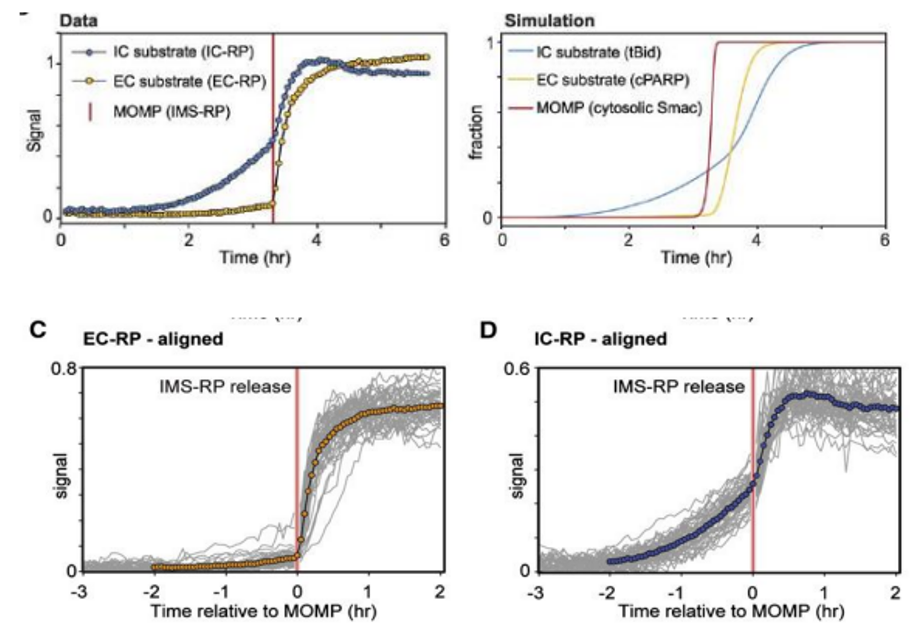
\includegraphics[width = 0.6\textwidth]{figs/simul-cells.png}
\end{figure}

En el artículo se ha estudiado el proceso de apoptosis de células tumorales tras administrar una droga (un fármaco). Las proteínas se han marcado fluorescentemente, y se puede ver cómo cambian las distintas proteínas tras la administración. Esto se puede simular de forma precisa, pero estas simulaciones se corresponden a experimentos de los que se obtiene una media poblacional. Las proteínas individuales tienen fluctuaciones en el tiempo. Todas las fluctuaciones están promedidadas, por lo que el modelo de ecuaciones diferenciales determinista simula el promedio de las células. En los experimentos se mide la fluorescencia total en la célula, no su localización subcelular.

En algunos sistemas, como el desarrollo embrionario, las \textbf{coordenadas espaciales} son cruciales. Las células se diferencian según su posición, y los genes se expresan en "oleadas". Para modelar estos sistemas, se usan \textbf{ecuaciones diferenciales parciales (EDPs),} que consideran tanto el tiempo como el espacio.

\begin{figure}[h]
\centering
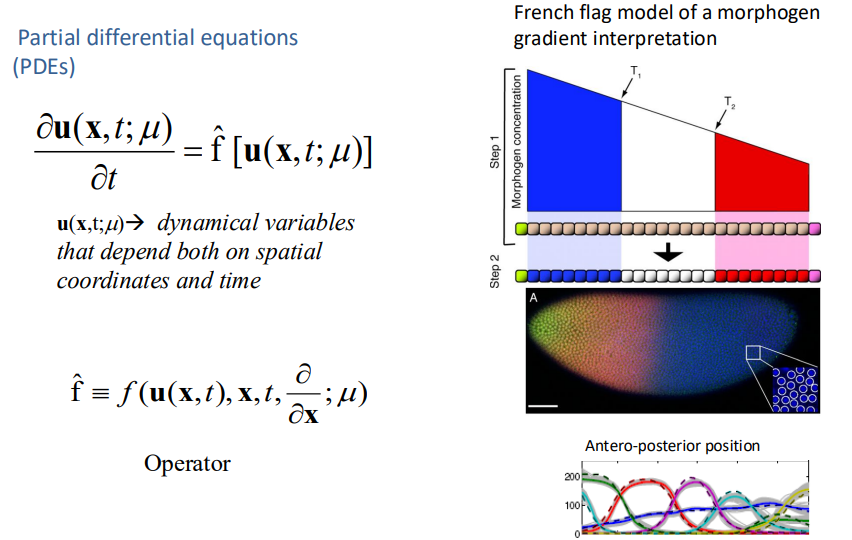
\includegraphics[width = 0.6\textwidth]{figs/pde-embryo.png}
\end{figure}

\section{Procesos dinámicos simples celulares: crecimiento celular, dilución proteica y degradación}
\subsection{Crecimiento celular}
El crecimiento celular es un proceso dinámico donde el número de células $N(t)$ aumenta con el tiempo. La velocidad de crecimiento se describe con la ecuación:
$$\frac{dN}{dt} = rN$$
donde r es la tasa de crecimiento y $N(t)$ el número de células en el tiempo t. Se trata de un sistema lineal con una sola variable. Los pasos para resolver la ecuación son:
\begin{enumerate}
\item Separar variables:
$$\frac{dN}{N} = r dt$$
\item Integrar ambos lados:
$$\int \frac{dN}{N} = \int r \cdot dt \rightarrow ln N = r t + C$$
\item Aplicar exponencial
$$N(t) = e^{rt + C} = e^C \cdot e^{rt}$$
\item Definir la constante $e^C = N(0)$, el número inicial de células o condiciones iniciales:
$$N(t) = N(0) \cdot e^{rt}$$
\end{enumerate}

El tiempo de duplicación $T_{div}$ indica el tiempo necesario para que $N(t)$ se duplique. Se calcula como:
$$N(T_{div}) = 2N(0) = N(0) \cdot e^{r \cdot T_{div}}$$
Dividiendo por $N(0)$:
$$ e^{r \cdot T_{div}} = 2 \rightarrow r \cdot T_{div} = ln 2 \rightarrow r = \frac{ln 2}{T_{div}}$$

\subsubsection{Ejercicio: Malthusian growth of bacteria}
Con el modelo lineal de crecimiento celular, ¿cuánto tiempo tardará una sola bacteria que se divide a un ritmo constante en llenar todos los océanos del mundo?. Datos: Supongamos que las bacterias tienen un volumen de 1 micrómetro cúbico y se dividen cada 30 minutos (valores típicos en \textit{E. coli}). El volumen estimado de todos los océanos es de $292.131.000 km^3$.

Podemos redondear el volumen de todos los océanos como:
$$V_{oceans} = 300.000.000 km^3 = 3 \cdot 10^8 km^3 = 3 \cdot 10^8 \cdot 10^{27} \mu m^3 = 3 \cdot 10^{35} \mu m^3$$
Los datos de una bacteria son:
$$V_{bacteria} = 1 \mu m^3$$
$$T_{div} = 30 mins = 0,5 h$$
Como partimos de una bacteria, la condición inicial es $c_0 = 1$.

Queremos que las bacterias colonicen todos los océanos. Para ello, se busca obtener el siguiente número de bacterias:
$$N = \frac{V_{oceans}}{V_{bacteria}} = \frac{3 \cdot 10^{35} \mu m^3}{1 \mu m^3} = 3 \cdot 10^{35}$$

Tenemos las siguientes fórmulas:
$$r = \frac{ln 2}{T_{div}} $$
$$N(t) = N(0) \cdot e^{rt} \rightarrow N(t) = e^{rt}$$

Sustituyendo, quedaría lo siguiente:
$$3 \cdot 10^{35} = e^{\frac{ln 2}{0,5} \cdot t} \rightarrow ln 3 + 35 \cdot ln 10 = \frac{ln 2}{0,5} \cdot t \rightarrow t = 58 h$$

Este modelo no es útil porque está demasiado simplificado. Hay que tener en cuenta los nutrientes, las restricciones espaciales, etc. 

%05/02 - Raúl Guantes
\subsection{Dilución proteica}
Durante el crecimiento celular, las proteínas se diluyen debido al aumento del volumen celular. Este fenómeno ocurre porque, al dividirse una célula, las proteínas se distribuyen entre las dos células hijas, reduciendo su concentración en cada una de ellas.

\subsubsection{Modelización de la dilución proteica}
Sea $P(t)$ el número de proteínas por célula en el tiempo $t$. Consideremos que partimos inicialmente de $P(0) = 8$ proteínas por célula y $N(0) = 1$ célula. 
Tras un tiempo de división $T_{div}$, la célula se divide en dos células hijas, y las proteínas se distribuyen aproximadamente en partes iguales entre ellas. Por tanto:
$$P(T_{div}) = \frac{P(0)}{2}$$
Tras $n$ divisiones celulares, el número de proteínas por célula se reduce a:
$$P(nT_{div}) = \frac{P(0)}{2^n}$$
Generalizando para cualquier tiempo $t$, el número de proteínas por célula sigue la relación:
$$P(t) = P(0) \cdot 2^{-\frac{t}{T_{div}}}$$

\subsubsection{Relación con el crecimiento exponencial de la población}
El número total de células $N(t)$ crece exponencialmente con el tiempo:
$$N(T_{div}) = N(0) \cdot e^{r \cdot T_{div}}$$
donde $r = ln 2 / T_{div}$ es la tasa de crecimiento. 

El número total de proteínas en la población $P^{tot}(t)$ se mantiene constante, ya que las proteínas no se crean ni se destruyen, solo se distribuyen entre las células hijas:
$$P^{tot}(t) = P^{tot}(0)$$
Por tanto, el número de proteínas por célula $P(t)$ se puede expresar como:
$$P(t) = \frac{P^{tot}(t)}{N(t)} = \frac{P^{tot} (0)}{N(0) \cdot e^{\frac{ln 2}{T_{div}} \cdot t}} = P(0) \cdot e^{-\frac{ln 2}{T_{div}} \cdot t}$$

\subsubsection{Ecuación diferencial de la dilución proteica}
La dinámica de la dilución proteica se describe mediante una ecuación diferencial que relaciona la tasa de cambio de $P(t)$ con el tiempo:
$$\frac{dP}{dt} = -\frac{ln 2}{T_{div}} \cdot P(t)$$

Es importante distinguir entre:
\begin{itemize}
\item \textbf{Ecuación diferencial:} describe cómo cambia $P(t)$ con el tiempo. En este caso, indica que la tasa de cambio de $P(t)$ es proporcional a $P(t)$ misma, con una constante de proporcionalidad negativa $- ln 2/T_{div}$.
\item \textbf{Solución de la ecuación diferencial:} proporciona la expresión explícita de $P(t)$ en función del tiempo.
\end{itemize}

En este contexto de dilución proteica, la tasa de cambio de la cantidad de proteínas por célula $P(t)$ se puede expresar en términos de una \textbf{constante de dilución} $\delta_{dil}$, definida como:
$$ \delta_{dil} = \frac{ln 2}{T_{div}}$$
Por lo tanto, la ecuación diferencial que describe la dilución proteica se reescribe como:
$$\frac{dP}{dt} = -\frac{ln 2}{T_{div}} \cdot P(t) = -\delta_{dil} \cdot P(t)$$
Esta ecuación indica que la cantidad de proteínas por célula disminuye exponencialmente con el tiempo debido a la división celular.

\subsection{Degradación activa de proteica}
Además de la dilución, las proteínas también pueden sufrir degradación activa, un proceso en el que las proteínas son descompuestas o eliminadas de la célula. En aproximadamente el 80\% de los casos medidos, la cantidad de proteínas disminuye de forma exponencial debido a este proceso.

\subsubsection{Modelización de la degradación}
La degradación activa se modela mediante una tasa de degradación $\delta_{deg}$, que describe cómo la cantidad total de proteínas $P^{tot}(t)$ en la población celular disminuye con el tiempo:
$$P^{tot}(t) = P^{tot}(0) \cdot e^{-\delta_{deg}\cdot t}$$

La ecuación diferencial que describe este proceso es:
$$ \frac{dP^{tot}}{dt} = -\delta_{deg} \cdot P^{tot}$$

\subsubsection{Combinación de dilución y degradación}
Cuando tanto la dilución como la degradación están presentes, la cantidad de proteínas por célula $P(t)$ se ve afectada por ambos procesos. Para modelar esto, combinamos las contribuciones de la dilución y la degradación.
\begin{enumerate}
\item \textbf{Cantidad total de proteínas}
$$P^{tot}(t) = P^{tot}(0) \cdot e^{-\delta_{deg} \cdot t}$$

\item \textbf{Número de células}
$$N(t) = N(0) \cdot e^{\frac{ln 2}{T_{div}} \cdot t}$$

\item \textbf{Proteínas por célula}
$$P(t) = \frac{P^{tot} (t)}{N(t)} = \frac{P^{tot}(0) \cdot e^{-\delta_{deg} \cdot t}}{N(0) \cdot e^{\frac{ln 2}{T_{div}} \cdot t}} = P(0) \cdot e^{-(\delta_{deg} + \frac{ln2}{T_{div}})t}$$
donde $P(0) = \frac{P^{tot}(0)}{N(0)}$ es la cantidad inicial de proteínas por célula.

\item \textbf{Tasa de cambio combinada}

Definimos la \textbf{tasa de disminución total} $\delta$ como la suma de la tasa de degradación activa $\delta_{deg}$ y la tasa de dilución $\delta_{dil}$:
$$\delta = \delta_{deg} + \delta_{dil}$$
Por tanto, la expresión para $P(t)$ se simplifica a:
$$P(t) = P(0) \cdot e^{-\delta \cdot t}$$
Y la ecuación diferencial que describe la dinámica combinada es:
$$\frac{dP}{dt} = -\delta P$$
\end{enumerate}

La constante $\delta$ representa la tasa efectiva de disminución de proteínas por célula, teniendo en cuenta tanto la degradación activa como la dilución debida al crecimiento celular. Un valor mayor de $\delta$ indica una disminución más rápida de la cantidad de proteínas por célula.

\subsubsection{Vida media}
La vida media ($T_{1/2}$) es el tiempo necesario para que la concentración de una sustancia (en este caso, proteínas) se reduzca a la mitad de su valor inicial. Matemáticamente, esto se expresa como:
$$P(T_{1/2}) = \frac{P(0)}{2}$$

Partiendo de la ecuación que describe la disminución exponencial de la concentración de proteínas:
$$P(t) = P(0) \cdot e^{-\delta t}$$
Sustituyendo $t = T_{1/2}$ y $P(T_{1/2}) = \frac{P(0)}{2}$, obtenemos:
$$\frac{P(0)}{2} = P(0) \cdot e^{-\delta \cdot T_{1/2}}$$
Simplificando $P(0)$ en ambos lados:
$$\frac{1}{2} = e^{-\delta \cdot T_{1/2}}$$
Aplicando el logaritmo neperiano a ambos lados:
$$ln(\frac{1}{2}) = - \delta \cdot T_{1/2}$$
Resolviendo para $T_{1/2}$:
$$T_{1/2} = \frac{ln 2}{\delta}$$
Por lo tanto, la constante de disminución $\delta$ se relaciona con la vida media mediante:
$$\delta = \frac{ln 2}{T_{1/2}}$$

\subsection{Combinación: producción y degradación de proteínas}
En muchos sistemas biológicos, las proteínas no solo se degradan, sino que también se producen activamente. Para modelar este proceso, introducimos:
\begin{itemize}
\item $\alpha$: la \textbf{tasa de producción} de proteínas, con unidades de proteínas por unidad de tiempo.
\item $\delta$: la \textbf{tasa de disminución total}, que incluye tanto la degradación activa como la dilución debida al crecimiento celular, con unidad de inversa de tiempo.
\end{itemize}
La dinámica de la cantidad de proteínas $P(t)$ se describe mediante la siguiente ecuación diferencial:
$$\frac{dP}{dt} = \alpha - \delta P$$

\subsubsection{Resolución de la ecuación diferencial}
Para resolver esta ecuación, seguimos los siguientes pasos:
\begin{enumerate}
\item \textbf{Separación de variables}
$$\frac{dP}{\alpha - \delta P} = dt$$

\item \textbf{Integración de ambos lados}
$$\int \frac{dP}{\alpha - \delta P} = \int dt$$

\item \textbf{Resolución de las integrales}

La integral del lado derecho es:
$$\int dt = t + cte$$

La integral del lado izquierdo requiere una sustitución. Sea $u = \alpha - \delta P$, entonces $du = - \delta dP$, y
$$\int \frac{dP}{\alpha - \delta P} = - \frac{1}{\delta} \int \frac{du}{u} = -\frac{1}{\delta} ln |u| + C = -\frac{1}{\delta} ln(\alpha - \delta P) + C$$

\item \textbf{Igualando ambas integrales}
$$-\frac{1}{\delta} ln (\alpha - \delta P) = t + C$$

\item \textbf{Despejando $P(t)$}

Multiplicamos ambos lados por $-\delta$:
$$ln(\alpha - \delta P) = -\delta t + C'$$
donde $C' = -\delta C$.

Aplicamos la exponencial a ambos lados:
$$\alpha - \delta P = e^{-\delta t + C'} = e^{C'} \cdot e^{-\delta t}$$

Despejamos $P(t)$:
$$P(t) = \frac{\alpha}{\delta} - \frac{e^{C'}}{\delta} e^{-\delta t}$$

\item \textbf{Determinación de la constante $C'$}

Aplicamos la condición inicial $P(0)$:
$$P(0) = \frac{\alpha}{\delta} - \frac{e^{C'}}{\delta}$$

Despejamos $e^{C'}$:
$$e^{C'} = \alpha - \delta P(0)$$

\item \textbf{Sustituyendo $e^{C'}$ en la solución}:
$$P(t) = \frac{\alpha}{\delta} - \frac{\alpha - \delta P(0)}{\delta} e^{-\delta t}$$
Y simplificando:
$$P(t) = \frac{\alpha}{\delta} (1 - e^{-\delta t}) + P(0) e^{-\delta t}$$
\end{enumerate}

\subsubsection{Estado estacionario}
Cuando $t\rightarrow \infty$, el término exponencial $e^{-\delta t}$ tiende a 0, y la cantidad de proteínas $P(t)$ alcanza un estado estacionario:
$P(t) \rightarrow \frac{\alpha}{\delta}$
Este valor representa el equilibrio entre la producción y la degradación de proteínas.




%05/02 - Raúl Guantes
\chapter{Sistemas dinámicos no lineales}
\section{Crecimiento logístico}
El crecimiento de las poblaciones está limitado por los recursos que están disponibles. Para ello, se debe añadir un parámetro nuevo, denominado como $k$, que indica la cantidad de recursos. Suponemos que la población tiene una tasa de crecimiento $r$ positiva. Además, contamos con $N(t)$, que es el número de células a un tiempo t. 

Suponiendo que hay una ecuación diferencial que dice cómo cambia la población con el tiempo en función de la variable y los parámetros r y k:
$$\frac{dN}{dt} = f(N; r, k)$$
Suponiendo que los recursos son ilimitados, $r N$. No obstante, si los recursos son limitados, entonces el tamaño depende de los recursos. Si la población es mayor que la disponibilidad de los recursos, la población debe disminuir y habrá células que mueran. SI el tamaño de la población es pequeño, hay recursos suficientes y la población crece. En otras palabras, la derivada es positiva o negariva según si la población crece o disminuye respectivamente. 
$$r N (1 - \frac{N}{k}$$
Esto se conoce como la ecuación de crecimiento logística. Esta ecuuación es no lineal porque N termina estando al cuadrado. 

$$N(t) = \frac{N(0) k}{N(0) + (k - N(0))e^{-rt}}$$
A tiempo infinito, la población tiende al valor de k, quedando en el equilibrio.
En estado de equilibrio, la derivada en función del tiempo da 0. 
$$0 = r N (1 - \frac{N}{K}) \begin{cases} 
N^1_{eq} = K \rightarrow \text{Estable} \\
N^2_{eq} = 0 \rightarrow \text{Inestable}
\end{cases}
$$

Para entender el comportamiento a tiempos largos (en equilibrio), hay que calcular puntos de equilibrio y la estabilidad. Si tenemos un sistema biológico de verdad, al medir a tiempos largos, siempre va a estar en un estado de equilibrio estable, al ser robustos a fluctuaciones. La estabilidad se puede deducir sin resolver la ecuación diferencial mediante dos formas: la forma gráfica y la forma matemática. 

\subsection{Cálculo de estabilidad de forma gráfica}
Con una sola variable, se pinta el denominado \textbf{plano de fases}. En el eje x está la variable, y en el y la derivada de la variable con respecto al tiempo. 
$$\frac{dN}{dt} = f(N) = rN - \frac{rN^2}{K}$$ 
Los puntos de corte son en 0 y en k, quedando una parábola invertida. Para calcular el máximo hay que poner la derivada en 0.
$$\frac{df}{dN} = 0 = r - \frac{2rN}{k} \rightarrow N = \rightarrow N = \frac{rk}{2r} = \frac{k}{2}$$

El punto de equilibrio en k es estable, porque N siempre va a converger a ese punto, ya que en un lado la función es positiva y en el otro lado negativa.

\subsection{Cálculo de estabilidad de forma matemática o por linealización}
La ventaja de este método es que se puede aplicar al número de variables que se quiera. Esta estabilidad se obtiene por linealización. 
Se busca analizar la función en un valor de equilibrio con una pequeña perturbación. 
$$N = N_{eq} + \Delta N$$
Al derivar:
$$\frac{d(N_{eq} + \Delta N)}{dt} = f(N_{eq} + \Delta N$$
$$(\frac{dN_{eq}}{dt} = 0) + \frac{d \Delta N}{dt}$$

$f(N)$ se aproxima por un polinomio según la serie de Taylor. En otras palabras, se aproxima:
$$f(N) \approx a + bN + cN^2 + dN^3 + \ldots$$ 
Vamos a usar eso para realizar una aproximación alrededor de un punto $N_0$. Para aproximar en una línea recta, debe pasar por ese punto y su pendiente debe ser la pendiente de la función, es decir, la derivada de la función y la variable.
$$a = f(N_0); b = \frac{df}{dN}; f = a + bN$$

$$f(N) \approx f(N_0) + \frac{df(N_0)}{dN} (N-N_0) + \frac{1}{2} \frac{d^2f(N_0)}{dN^2} (N-N_0)^2 + \ldots \frac{1}{n!} \frac{d^n(N_0)}{dN^n}(N-N_0)^n$$
Esta aproximación de Taylor se utiliza para aproximar la función $f(N_{eq} + \Delta N$ alrededor del punto $N_{eq}$. 
$$\frac{d \Delta N}{dt} = f(N_{eq} + \frac{df(N_{eq})}{dN} (N-N_{eq}) \rightarrow \frac{\Delta N}{dt} = f'(N_{eq} \Delta N$$

Si $f'(N_{eq}) > 0$, el punto de equilibrio es inestable, ya que aumentaría en el tiempo ($\Delta N(t) = \Delta N(0) \cdot e^{f'(N_{eq}) t}$). Si $f'(N_{eq}) < 0$, entonces el punto de equilibrio es estable.



\end{document}
